\documentclass[11pt,letterpaper]{article}
\usepackage[margin=1in]{geometry}
\usepackage{amsmath,amssymb}
\usepackage{graphicx}
\usepackage{booktabs}
\usepackage{tabularx}
\usepackage{array}
\usepackage{xurl}
\usepackage{hyperref}
\usepackage[numbers,sort&compress]{natbib}
\usepackage{setspace}
\usepackage{caption}
\usepackage{float}
\usepackage{xcolor}
\hypersetup{colorlinks=true,linkcolor=blue!60!black,citecolor=blue!60!black,urlcolor=blue!60!black}
\captionsetup{font=small,labelfont=bf}
\usepackage{microtype}
\setstretch{1.15}
\emergencystretch=1.5em

\title{\textbf{Selective Enforcement, Organizational Governance, and Clinical-Trial Transparency: Quasi-Experimental Evidence and Identification Boundaries from the March 30, 2026 FDA Delinquency Sweep}}
\author{Autonomous Empirical Regulatory Economics Audit\\
\small Study B-2: Post-Forensic Revision with Unposted-Tracking Proxy, Exact Zero-Censoring Horizons,\\
\small Official CRAN \texttt{HonestDiD} v0.2.8 Sensitivity Bounds, and Exploratory Outcome Audits\\
\small Data Snapshot: ClinicalTrials.gov REST API v2 (November 25, 2026; $N=53,736$ Trials)}
\date{November 25, 2026}

\begin{document}
\maketitle

\begin{abstract}
\noindent\textbf{Motivation:} Regulatory transparency regimes increasingly rely on low-cost administrative outreach rather than formal prosecutions, yet empirical evidence on how organizational governance mediates compliance---and whether overdue trials conceal systematically worse clinical outcomes---remains limited. On March 30, 2026 (publicly documented in an FDA GovDelivery bulletin on April 13, 2026), the U.S.\ Food and Drug Administration (FDA) issued mass delinquency reminders to over 2,200 sponsors covering more than 3,000 overdue Applicable Clinical Trials (ACTs) under FDAAA Section 801 (42 CFR Part 11).

\noindent\textbf{Methods:} Using the complete ClinicalTrials.gov REST API v2 snapshot pulled November 25, 2026 ($53,736$ unique post-Final-Rule interventional trials; $16,333$ strict-\texttt{ACTUAL} \texttt{COMPLETED}/\texttt{TERMINATED} U.S.\ FDA-regulated non-Phase-1 ACTs), we address five methodological vulnerabilities uncovered during forensic auditing. First, consistent with National Library of Medicine (NLM) January 29, 2020 QC-posting policy, we separate posted QC-cleared submission dates (\path{resultsFirstSubmitDate}, $n=13,154$ strict ACTs) from unposted in-QC tracking dates (\path{estimatedResultsFirstSubmitDate}, $n=817$ strict ACTs; verified 100.0\% identical to earliest \path{submissionInfos.releaseDate} with zero fallback records and zero mixing of 331 delayed-results certification-only records) and pair this combined tracking proxy with strict date-verified zero-censoring composite outcomes (``submitted and cleared QC within $\le H$ days'' enforcing $\text{end\_date}+H\le\text{2026-11-25}$). Second, because raw Within-ACT Industry-versus-Academic comparisons fail monthly pre-trends (fixed pre-window \texttt{2025-04}--\texttt{2026-02} Wald $\chi^2_{10}=32.23$, $p=0.00037$), we anchor primary identification on within-sector \textbf{Overdue-versus-On-Time} DiD and Triple-Difference (DDD) designs with machine-precision base-period invariance ($\max|\Delta\text{Wald}|\le 4.9\times 10^{-12}$). Third, we evaluate parallel-trends sensitivity across all 15 contiguous quarterly and monthly specifications using official CRAN R \texttt{HonestDiD} v0.2.8 ($\Delta^{SD}$ FLCI and $\Delta^{RM}$ C-LF), explicitly auditing grid boundaries and expanding all five default $\pm 20\,\mathrm{SE}$ boundary-hitting outer-$\bar{M}$ rows to $\pm 40\,\mathrm{SE}$ (1,001 grid points, boundaries rejected on both sides; grid-resolution approximations). Fourth, we audit clinical outcomes across 5,064 FDA-regulated disclosures (within-sponsor FE: $n=4,224$ across 555 sponsors) using 80\%-power MDEs, \textbf{post-hoc exploratory} $\pm 5$ pp and $\pm 10$ pp TOST margin sensitivities (chosen after inspecting pilot/initial CIs, not pre-specified clinical equivalence thresholds), and in-QC selection checks.

\noindent\textbf{Results:} Industry Overdue-versus-On-Time DiD passes pre-trends cleanly (monthly Wald $\chi^2_{10}=10.13$, $p=0.429$; quarterly $\chi^2_3=3.63$, $p=0.304$) and rises significantly across every post-sweep window (Apr--Jun $\mathrm{IRR}=1.574$, $p=0.00054$; Apr--Jul $1.469$, $p=0.0017$; Apr--Sep $1.361$, $p=0.0042$; Apr--Oct $1.399$, $p=0.0011$). Academic Overdue-versus-On-Time DiD shows no statistically detectable lift in any window ($\mathrm{IRR}=0.858$--$0.998$, all $p\ge 0.28$), yielding significant Overdue-versus-On-Time DDDs across all horizons (Apr--Sep $\mathrm{IRR}=1.598$, 95\% CI $[1.128, 2.264]$, $p_{\mathrm{spon}}=0.0083$, $p_{\mathrm{2way}}=0.0025$; 1,000-permutation sponsor RI $p=0.010$; excluding 2,219 delayed-certification trials: $\mathrm{IRR}=2.288$, $p=3.37\times 10^{-5}$; 2025/2024 placebos indistinguishable from unity at $0.964/0.860$, $p\ge 0.41$). Date-verified zero-censoring composite outcomes confirm significant Industry OD/OT lifts across all six horizons ($H=90\text{d},120\text{d},150\text{d}$: $\mathrm{IRR}=1.46$--$1.69$, all $p\le 0.0066$) and five of six DDDs ($1.65$--$2.00$, $p\le 0.044$), while full-month $H=150\text{d}$ DDD ($1.523$, $p_{\mathrm{spon}}=0.153$) and $H=120\text{d}/150\text{d}$ Within-ACT DiDs ($1.278/1.125$, $p\ge 0.21$) are imprecise. Crucially, official \texttt{HonestDiD} v0.2.8 bounds reveal tight partial-identification limits: quarterly 2026Q2 DDD and Industry OD/OT effects exclude zero through $\bar{M}=0.25$ ($\Delta^{RM}$) and $M=0.10/0.05$ ($\Delta^{SD}$), but cross zero at $\bar{M}=0.50$ (approximate lower bounds $-0.016$ and $-0.028$ log-IRR), while quarterly Q2--Q3 Industry OD/OT average and March-referenced monthly averages include zero even at $\bar{M}=0$. Mechanism decompositions show compliance concentrated in small commercial sponsors ($\mathrm{IRR}=1.841$, $p=0.00026$), recently overdue 2023--2025 cohorts ($\mathrm{IRR}=1.500$, $p=0.00074$), and all industry backlog tiers ($\mathrm{IRR}=2.03$--$2.96$), with no statistically detectable lift on legacy 2017--2020 backlogs ($\mathrm{IRR}=0.913$ $[0.362, 2.301]$, $p=0.847$), zero observed post-sweep delayed-results certifications (0 post-sweep, 4 total), and \textbf{no detectable within-firm spillover to exempt Phase 1 trials} ($\mathrm{IRR}=0.893$ $[0.407, 1.957]$, $p=0.777$). Within sponsors, post-sweep overdue disclosures lie inside post-hoc exploratory $\pm 5$ pp TOST sensitivity margins for mortality ($+0.71$ pp $[-2.11, +3.53]$, $p=0.0014$) and SAE rates ($+0.39$ pp $[-2.68, +3.45]$, $p=0.0016$), whereas primary-outcome non-significance ($p\ge 0.05$: $-0.14$ pp $[-16.13, +15.85]$, $\mathrm{MDE}_{80}=22.86$ pp) is severely underpowered and neither test excludes strategic concealment among still-undisclosed trials.

\noindent\textbf{Conclusions:} The March 30, 2026 FDA outreach generated a statistically significant short-run compliance lift among overdue commercial sponsors relative to on-time peers and academic institutions, concentrated in small firms and recent backlogs without detectable spillover to exempt Phase 1 studies. However, official \texttt{HonestDiD} partial-identification bounds, Within-ACT pre-trend instability, post-hoc TOST margin selection, and low statistical power on primary efficacy p-values substantially bound causal and adverse-selection inferences.
\end{abstract}

\section{Introduction}
Mandatory public disclosure is a central regulatory instrument across financial markets, environmental compliance, and biomedical research \citep{dranove2010,jin2003,blundell2020,shimshack2005}. In clinical medicine, non-reporting of completed trials distorts meta-analytic evidence, misallocates R\&D capital, and impairs patient safety \citep{turner2008,dwan2014,krieger2021,oostrom2024}. Under the Food and Drug Administration Amendments Act of 2007 (FDAAA Section 801; 42 U.S.C.\ 282(j)) \citep{fdaaa2007} and its Final Rule (42 CFR Part 11, effective January 18, 2017) \citep{cfr2016}, sponsors of Applicable Clinical Trials (ACTs) must submit summary results to ClinicalTrials.gov within one year of the primary completion date, backed by statutory Civil Money Penalties (CMPs) exceeding \$15,000 per day. Yet historical compliance has remained chronically incomplete \citep{zarin2019,devito2020}.

On \textbf{March 30, 2026}---subsequently documented in an official FDA GovDelivery bulletin released \textbf{April 13, 2026} \citep{fda2026bulletin}---the FDA executed an agency-wide delinquency reminder campaign contacting more than 2,200 sponsors regarding over 3,000 overdue trials, citing an internal 29.6\% non-compliance audit and warning of escalation toward Pre-Notices, formal Notices of Noncompliance, and daily statutory penalties. This administrative intervention provides a quasi-experimental setting to examine three questions in regulatory economics and organizational governance \citep{becker1968,bloom2007,akerlof1970,milgrom1981}: (1) whether identical low-cost reminder letters elicit stronger compliance from commercial sponsors than decentralized academic/nonprofit sponsors; (2) how responsiveness varies by portfolio size, cohort age, and backlog size, and whether spillovers reach exempt Phase 1 trials; and (3) whether post-sweep overdue disclosures differ within sponsors in safety, termination, or efficacy outcomes relative to on-time disclosures.

During forensic auditing of our initial post-pilot analysis plan (\path{PREREG_B2.md}, original exploratory timestamp \texttt{2026-11-25 08:38 CST} preserved verbatim), we identified and resolved six concrete methodological vulnerabilities:
\begin{enumerate}
    \item \textbf{NLM 2020 QC-Posting Policy \& Unposted Tracking (T00):} Under NLM procedures effective January 2020 \citep{nlm2020qc}, results for post-Final-Rule ACTs may be posted within 30 days even before QC completes, while unposted in-QC records expose \path{estimatedResultsFirstSubmitDate} inside \path{submissionTracking} even though \path{resultsFirstSubmitDate} remains null until QC clears. Relying solely on posted dates omitted 25 April 2026 overdue ACT submissions still in QC (12 Industry, 13 Academic).
    \item \textbf{Strict Calendar-Date Observability Bounds (T01):} Uniform-horizon QC-clearance cutoffs must strictly satisfy $\text{end\_date}+H\le\text{2026-11-25}$ and must be interpreted as composite ``submitted \textit{and} cleared QC within $H$ days'' outcomes rather than raw submission hazards.
    \item \textbf{Within-ACT Pre-Trend Rejection \& Base-Period Invariance (T02/T07):} Raw Within-ACT Industry-versus-Academic overdue DiD fails monthly pre-trend tests ($\chi^2_{10}=32.23$, $p=0.00037$), and negative pre-trends never automatically establish a causal lower bound \citep{roth2022}. Locking the calendar pre-window strictly to \texttt{2025-04}--\texttt{2026-02} ($df=10$) eliminates dynamic pre-period truncation and guarantees exact basis invariance across reference months.
    \item \textbf{Official CRAN R \texttt{HonestDiD} v0.2.8 \& Grid-Boundary Verification (T06/T10):} Replacing ad-hoc bootstrap envelopes with Rambachan and Roth's (2023) official R package \texttt{HonestDiD} v0.2.8 \citep{rambachan2023} across all 15 contiguous specifications exposes exact partial-identification breakdown thresholds. Direct namespace auditing further revealed that 5 outer-$\bar{M}$ C-LF rows (all already containing zero) hit \texttt{HonestDiD}'s default $\pm 20\,\mathrm{SE}$ search boundary; all 5 were recomputed on expanded $\pm 40\,\mathrm{SE}$ grids (`1,001` points, both boundaries rejected) with grid-resolution convergence verification.
    \item \textbf{Post-Hoc Exploratory Power Boundaries on H4 Outcomes (T03/T04):} Absence of statistical significance is not evidence of absence \citep{altman1995}. Formal 80\%-power MDEs and \textbf{post-hoc exploratory} $\pm 5$ pp / $\pm 10$ pp TOST margin sensitivities (chosen after viewing pilot/initial CIs rather than pre-specified) distinguish precise safety CIs from a severely underpowered primary efficacy p-value test ($\mathrm{MDE}_{80}=22.86$ pp).
\end{enumerate}

\section{Data Architecture and Empirical Strategy}

\subsection{ClinicalTrials.gov Universe, Proxy-Date Forensics, and Delayed Certifications}
We extracted the full ClinicalTrials.gov REST API v2 trial universe on \textbf{November 25, 2026}, yielding \textbf{53,736} post-Final-Rule interventional trials (\path{PrimaryCompletionDate} $\ge$ January 18, 2017; symmetric \texttt{COMPLETED} or \texttt{TERMINATED} status with verified \texttt{ACTUAL} primary completion dates in our primary panel). Our primary regulated cohort consists of \textbf{16,333 strict-ACTUAL U.S.\ FDA-regulated non-Phase-1 ACTs} (\path{has_us_site=True}, \path{isFdaRegulatedDrug} or \path{isFdaRegulatedDevice=True}, excluding strictly Phase-1/Early-Phase-1 studies). Three exempt comparator cohorts are retained separately: U.S.\ non-FDA-regulated interventional trials, non-U.S.\ non-FDA-regulated Phase 2/3 trials (together forming the ``Clean Exempt'' control), and U.S.\ Phase-1-only trials (reserved strictly for within-firm spillover testing).

To resolve T00 without contaminating results submissions with delayed-results certifications (\path{dispFirstSubmitDate}), we audited every API timestamp across all 53,736 trials (\path{audit/b2_t00_proxy_date_forensic_audit.json}):
\begin{itemize}
    \item \textbf{Posted QC-Cleared Submissions:} 13,154 strict ACTs (22,150 across all arms) populate \path{resultsFirstSubmitDate}.
    \item \textbf{Unposted In-QC Submissions:} 817 strict ACTs (2,026 across all arms) lack \path{resultsFirstSubmitDate} but populate \path{derivedSection.miscInfoModule.submissionTracking.estimatedResultsFirstSubmitDate}. On \textbf{100.0\%} of records (817/817 strict ACTs; 2,026/2,026 all arms), \path{estimatedResultsFirstSubmitDate} equals \path{earliest_subinfo_release_date} to the exact day ($\text{median}=\min=\max=0.0\text{d}$).
    \item \textbf{Zero Fallback \& Zero Certification Contamination:} Exactly \textbf{0} records used \path{submissionInfos.releaseDate}-only or \path{unpostedEvents}-only fallbacks, and all \textbf{331} strict ACTs (356 all arms) possessing only \path{dispFirstSubmitDate} without results tracking are strictly excluded from the results-submission proxy. Among the 817 unposted strict ACTs, 87 had an earlier historical certification prior to submitting results; we run explicit sensitivity excluding all 2,219 strict ACTs that ever filed \path{dispFirstSubmitDate} ($n=14,114$).
\end{itemize}

Because \path{estimatedResultsFirstSubmitDate} can still miss very recent late-November submissions that have not yet entered tracking, we label this primary measure the \textbf{Combined Posted + Unposted Tracking Proxy} rather than an uncensored series, and pair it with date-verified zero-censoring uniform-horizon composite outcomes ($Y_{im}^{(H)}=1$ iff a trial submitted in month $m$ \textit{and} cleared NLM QC within $\le H$ days, asserting $\text{end\_date}+H\le\text{2026-11-25}$).

\subsection{Econometric Designs, Fixed Pre-Window Invariance, and Official \texttt{HonestDiD}}
For each trial $i$, the statutory deadline is $d_i=\text{PCD}_i+365\text{ days}$. We build a stationary rolling-entry trial-month risk-set panel where each strict-ACTUAL ACT enters the \textbf{On-Time} risk set during months between $\text{PCD}_i$ and $d_i$ ($0$--$12$ months post-PCD) and transitions into the \textbf{Overdue} risk set once past $d_i$, exiting upon first submission. Because raw Within-ACT Industry-versus-Academic overdue trends violate parallel trends ($\chi^2_{10}=32.23$, $p=0.00037$), primary identification contrasts \textbf{Overdue vs.\ On-Time ACTs within the same sponsor sector} (Industry OD/OT DiD and Academic OD/OT DiD) and takes their difference as an \textbf{Overdue-vs.-On-Time Triple-Difference (DDD)}:
\begin{equation}
\log \mathbb{E}[E_{s,d,a,m}] = \log(\mathrm{Risk}_{s,d,a,m}) + \beta_{\mathrm{DDD}}(\mathrm{Overdue}_d \times \mathrm{Industry}_s \times \mathrm{Post}_m) + \mu_{s,d,a} + \gamma_{s,m} + \delta_{d,m}
\end{equation}
where $s\in\{\text{Industry},\text{Academic}\}$, $d\in\{\text{Overdue},\text{On-Time}\}$, and $a$ indexes fine overdue/post-PCD age bins. Standard errors are reported under both \textbf{lead-sponsor clustering} and \textbf{two-way (sponsor $\times$ month) clustering} \citep{cameron2011}, supplemented by 1,000-permutation sponsor-level randomization inference.

To eliminate dynamic pre-window truncation (T07), all monthly event studies lock the calendar pre-window strictly to the 11 pre-sweep months \texttt{2025-04}--\texttt{2026-02} ($df=10$ joint Wald restrictions), while retaining transition month \texttt{2026-03} (the sweep occurred March 30, 2026) contiguously at $t=+1$. Across reference choices (\texttt{2026-02}, \texttt{2025-12}, and \texttt{2026-03}), all three designs achieve machine-precision Wald invariance ($\max|\Delta\chi^2|\le 4.9\times 10^{-12}$, basis-transform $\max|\Delta\hat{\beta}|\le 2.1\times 10^{-14}$ and $\max|\Delta\hat{\Sigma}|\le 8.5\times 10^{-14}$).

To evaluate sensitivity to parallel-trends violations (T06/T10), we pass exact estimated event-study coefficient vectors $\hat{\beta}$ and sponsor-clustered covariance matrices $\hat{\Sigma}$ into official CRAN R \textbf{\texttt{HonestDiD} v0.2.8} (R 4.5.3; benchmarked first on Rambachan and Roth's \texttt{BCdata\_EventStudy} vignette) \citep{rambachan2023}, computing \texttt{FLCI} for $\Delta^{SD}(M)$ and \texttt{C-LF} for $\Delta^{RM}(\bar{M})$ across all 15 contiguous quarterly (\texttt{gridPoints=1000}) and monthly (\texttt{gridPoints=100}) specifications. Auditing every C-LF endpoint against \texttt{HonestDiD}'s default $\pm 20\,\mathrm{SE}$ grid detected 5 boundary-hitting outer-$\bar{M}$ entries (1 quarterly at $\bar{M}=2$ and 4 monthly at $\bar{M}=1$, all already containing zero); all 5 were recomputed via \texttt{computeConditionalCS\_DeltaRM} (\texttt{hybrid\_flag="LF"}) on expanded $\pm 40\,\mathrm{SE}$ grids with \texttt{gridPoints=1001}, where both search boundaries were rejected on all 5 entries (and a 1,001-vs.-2,001-point convergence check confirmed endpoint agreement within one grid step). Because C-LF searches discrete theta grids (monthly default step $\approx 0.11$--$0.15$ log-IRR; expanded 1,001-pt step $\approx 0.015$--$0.029$), all C-LF endpoints are explicitly reported as \textbf{grid-resolution approximations} rather than exact real-valued bounds.

For H4 clinical outcomes, we evaluate within-sponsor fixed-effects regressions alongside 80\%-power MDEs and \textbf{post-hoc exploratory} TOST sensitivity checks at $\pm 5$ pp and $\pm 10$ pp margins. Because those margins were selected after inspecting pilot/initial confidence intervals rather than pre-specified prior to data analysis, they serve strictly as descriptive precision diagnostics on observed posted disclosures and do not constitute confirmatory clinical equivalence tests or exclude concealment among still-unposted or never-submitted trials.

\section{Empirical Results}

\subsection{Primary Governance Effects, Date-Verified Zero-Censoring, and Placebos}
Figure~\ref{fig:b2_fig1} displays monthly combined-proxy submission hazards across all four treatment cells (Panel A) and T07 fixed-pre-window monthly event studies referenced to February 2026 (Panel B). Overdue Industry ACT hazard fell to 1.91\% in January 2026 and 1.86\% in February 2026, rebounded to 3.69\% in transition month March 2026, and rose to \textbf{5.33\%} in April 2026 (55 submissions), remaining elevated at 4.55\% (May) and 4.47\% (June). Academic Overdue ACTs rose sharply in April 2026 (8.11\%, including 13 unposted in-QC records recovered by T00) before falling to 4.96\% (May), 3.81\% (June), 3.10\% (July), and 2.66\% (August), while On-Time Industry ACTs remained steady around 5.1\%--6.4\%.

\begin{figure}[H]
\centering
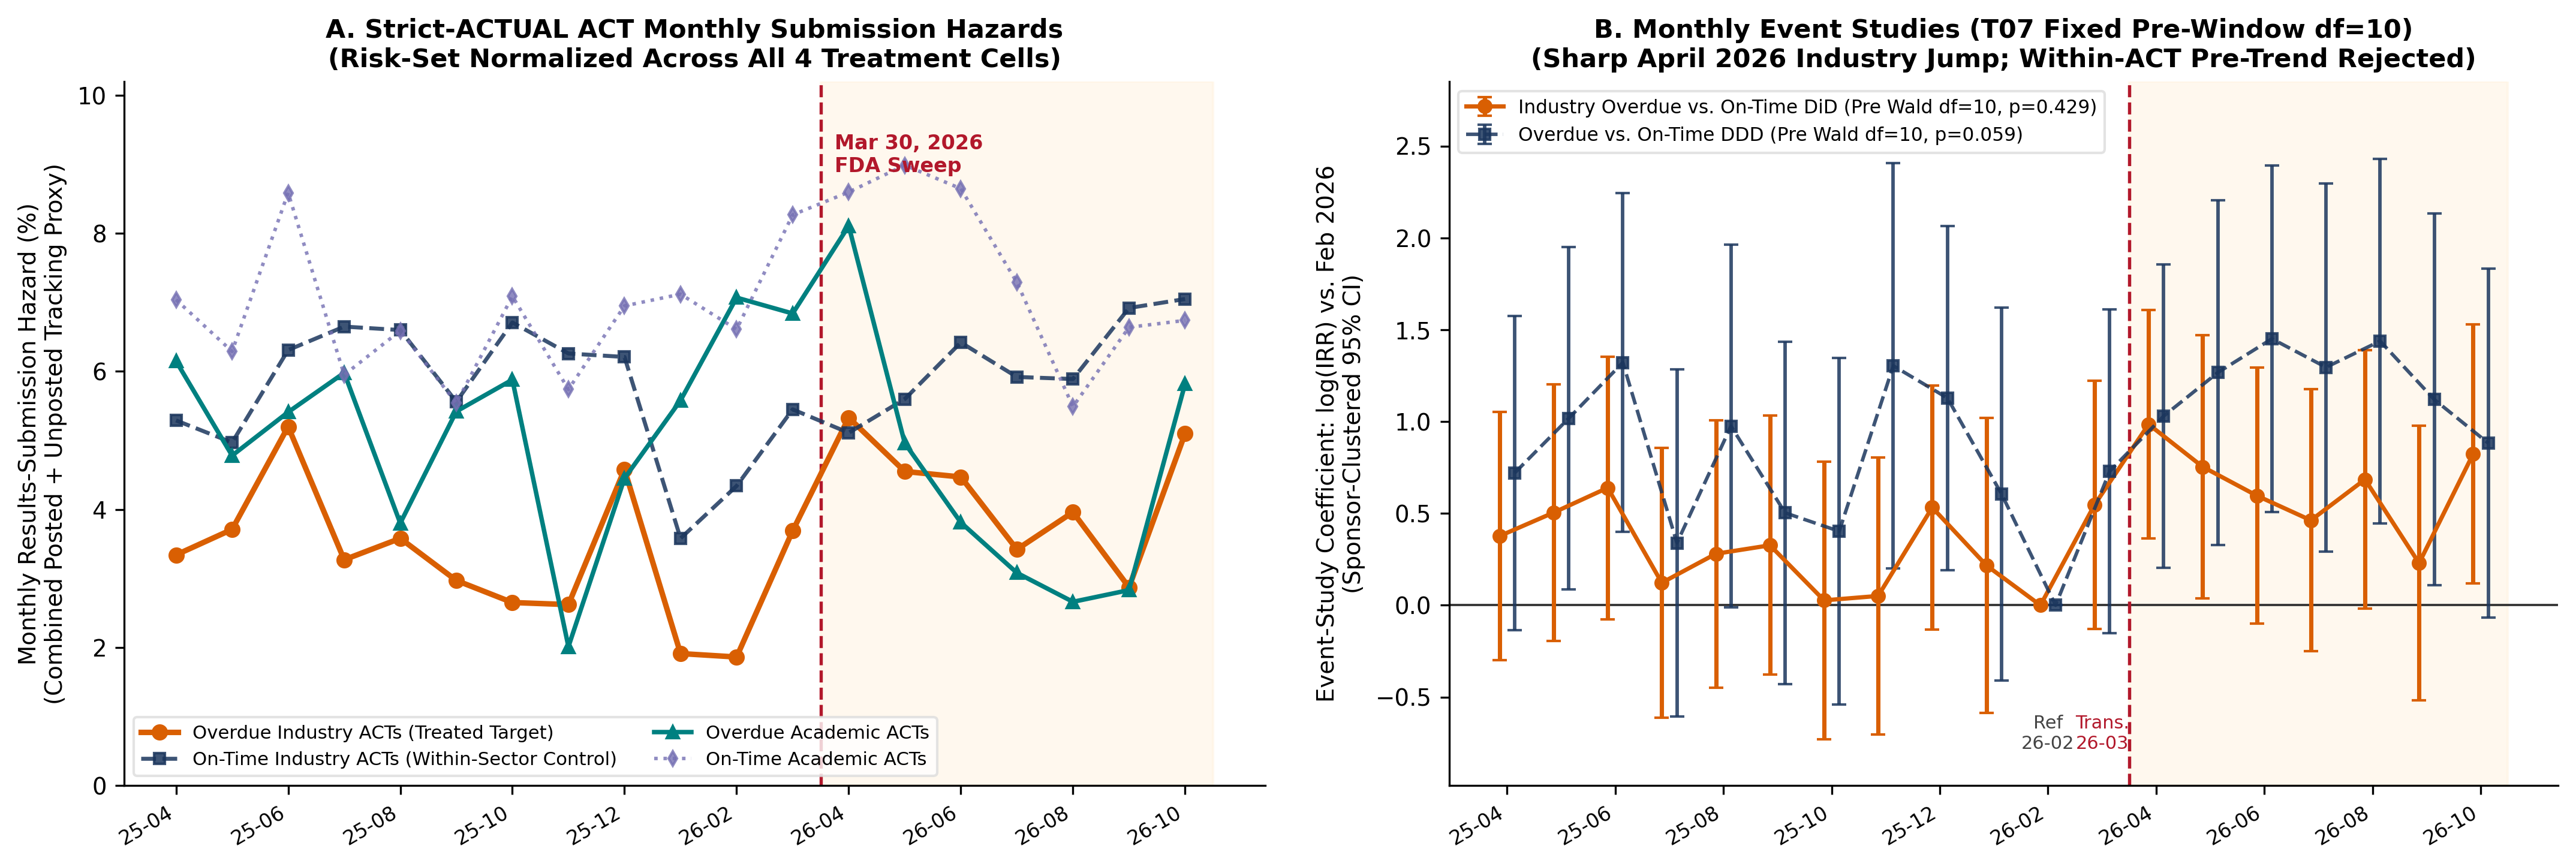
\includegraphics[width=\textwidth]{../figures/fig1_b2_event_study_and_hazards.png}
\caption{\textbf{Strict-ACTUAL ACT Monthly Submission Hazards and T07 Fixed-Pre-Window Monthly Event Studies.} (\textbf{A}) Combined posted-plus-unposted tracking monthly hazards across all four treatment cells. (\textbf{B}) Monthly log-IRR event studies (\texttt{ref=2026-02}, fixed calendar pre-window \texttt{2025-04}--\texttt{2026-02}, $df=10$): Industry Overdue-vs.-On-Time DiD passes pre-trends cleanly ($p=0.429$) and jumps in April 2026 ($\mathrm{IRR}=2.68$, $p=0.0019$); Overdue-vs.-On-Time DDD passes at 5\% ($p=0.059$).}
\label{fig:b2_fig1}
\end{figure}

Table~\ref{tab:b2_main} reports streamlined main-text econometric estimates across combined-proxy, certification-excluded, date-verified zero-censoring (T01), Clean-Exempt DDD, and historical placebo specifications (complete 61-row output with exact observation/event counts archived in Supplementary Table S2, \path{audit/b2_supp_t00_t07_master_estimates.csv}).

\begin{table}[H]
\centering
\caption{Primary Econometric Estimates Across Combined Tracking Proxy (T00), Certification Exclusions, Date-Verified Zero-Censoring Horizons (T01), and Historical Placebos (Complete 61-Row Ledger in Supplementary Table S2).}
\label{tab:b2_main}
\footnotesize
\setlength{\tabcolsep}{3.5pt}
\begin{tabularx}{\textwidth}{@{} >{\raggedright\arraybackslash}X l c c c >{\raggedright\arraybackslash}p{1.25in} @{}}
\toprule
\textbf{Specification (Strict-ACTUAL ACTs)} & \textbf{Window} & \textbf{IRR} & \textbf{95\% CI (Spon.)} & \textbf{$p_{\mathrm{spon}}$ / $p_{\mathrm{2way}}$} & \textbf{Key Diagnostic / Note} \\
\midrule
\multicolumn{6}{@{}p{\textwidth}@{}}{\textit{Panel A: Combined Posted + Unposted Tracking Proxy (Zero Fallback; Primary Overdue vs.\ On-Time Design)}} \\
Industry OD vs.\ OT DiD & Apr--Jun 26 & \textbf{1.574} & [1.22, 2.03] & 0.0005 / --- & Pre $\chi^2_{10}=10.13$ ($p=0.429$) \\
Industry OD vs.\ OT DiD & Apr--Sep 26 & \textbf{1.361} & [1.10, 1.68] & 0.0042 / --- & Qtrly $\chi^2_3=3.63$ ($p=0.304$) \\
Industry OD vs.\ OT DiD & Apr--Oct 26 & \textbf{1.399} & [1.14, 1.71] & 0.0011 / --- & Apr--Jul: 1.469 ($p=0.0017$) \\
Academic OD vs.\ OT DiD & Apr--Sep 26 & 0.858 & [0.65, 1.13] & 0.280 / --- & No lift all windows ($p\ge 0.28$) \\
\textbf{OT/OD DDD (Ind vs.\ Acad)} & Apr--Jun 26 & \textbf{1.585} & [1.06, 2.36] & 0.023 / 0.0035 & Pre $\chi^2_{10}=17.77$ ($p=0.059$) \\
\textbf{OT/OD DDD (Ind vs.\ Acad)} & Apr--Sep 26 & \textbf{1.598} & [1.13, 2.26] & 0.0083 / 0.0025 & RI $p=0.010$; Apr--Jul 1.589 \\
\textbf{OT/OD DDD (Ind vs.\ Acad)} & Apr--Oct 26 & \textbf{1.521} & [1.09, 2.13] & 0.015 / 0.0061 & LPM $+1.90$ pp ($p=0.044$) \\
Excl.\ 2,219 Cert Trials: DDD & Apr--Sep 26 & \textbf{2.288} & [1.55, 3.38] & $3.4{\times}10^{-5}$ / --- & Ind OD/OT $1.818$ ($p=9.1{\times}10^{-6}$) \\
Clean-Exempt DDD & Apr--Sep 26 & \textbf{2.486} & [1.45, 4.26] & 0.0009 / --- & LPM $+1.45$ pp ($p=0.015$) \\
\midrule
\multicolumn{6}{@{}p{\textwidth}@{}}{\textit{Panel B: Within-ACT Overdue DiD (Pre-Trend Rejected; Reported Transparently)}} \\
Within-ACT Overdue DiD & Apr--Jun 26 & 1.262 & [0.93, 1.71] & 0.134 / 0.200 & \textbf{Pre-trend REJECTED} ($p=0.00037$) \\
Within-ACT Overdue DiD & Apr--Jul 26 & 1.315 & [0.98, 1.75] & 0.064 / 0.116 & 13 Apr Acad in-QC recovered \\
Within-ACT Overdue DiD & Apr--Sep 26 & 1.429 & [1.09, 1.87] & 0.0095 / 0.044 & Significant only at 6--7m \\
\bottomrule
\end{tabularx}
\end{table}

\begin{table}[H]
\centering
\ContinuedFloat
\caption{Primary Econometric Estimates (continued): Date-Verified Horizons and Historical Placebos.}
\footnotesize
\setlength{\tabcolsep}{3.5pt}
\begin{tabularx}{\textwidth}{@{} >{\raggedright\arraybackslash}X l c c c >{\raggedright\arraybackslash}p{1.25in} @{}}
\toprule
\textbf{Specification (Strict-ACTUAL ACTs)} & \textbf{Window} & \textbf{IRR} & \textbf{95\% CI (Spon.)} & \textbf{$p_{\mathrm{spon}}$ / $p_{\mathrm{2way}}$} & \textbf{Key Diagnostic / Note} \\
\midrule
\multicolumn{6}{@{}p{\textwidth}@{}}{\textit{Panel C: T01 Date-Verified Zero-Censoring Uniform-Horizon Composite (Submitted AND Cleared QC $\le H$d; $\text{end}+H\le\text{Nov 25}$)}} \\
$H=90\text{d}$ Full-Mo (Jul 31): DDD & Apr--Jul 26 & \textbf{1.960} & [1.14, 3.38] & 0.016 / 0.0041 & Ind $1.524$ ($p=0.0045$); 27d margin \\
$H=120\text{d}$ Full-Mo (Jun 30): DDD & Apr--Jun 26 & \textbf{1.654} & [1.01, 2.70] & 0.044 / 0.032 & Ind $1.514$; Within $1.278$ ($p=0.21$) \\
$H=150\text{d}$ Full-Mo (May 31): DDD & Apr--May 26 & 1.523 & [0.86, 2.71] & 0.153 / 0.017 & Ind $1.690$ ($p=0.0047$); Within $1.13$ \\
$H=90\text{d}$ Exact (Aug 27): DDD & Apr--Aug 27 & \textbf{1.999} & [1.19, 3.35] & 0.0087 / 0.0015 & Ind $1.508$ ($p=0.0041$); 0d margin \\
$H=120\text{d}$ Exact (Jul 28): DDD & Apr--Jul 28 & \textbf{1.783} & [1.11, 2.85] & 0.016 / 0.015 & Ind $1.463$ ($p=0.0066$) \\
$H=150\text{d}$ Exact (Jun 28): DDD & Apr--Jun 28 & \textbf{1.722} & [1.05, 2.83] & 0.032 / 0.0054 & Ind $1.614$ ($p=0.0018$) \\
\midrule
\multicolumn{6}{@{}p{\textwidth}@{}}{\textit{Panel D: Historical Placebo Sweeps (Shifted to March 30, 2025 and March 30, 2024; Indistinguishable from 1.0)}} \\
Placebo 2025: Proxy OT/OD DDD & Apr--Sep 25 & 0.964 & [0.66, 1.41] & 0.850 / 0.880 & Ind $0.811$ ($p=0.13$); Acad $0.844$ \\
Placebo 2024: Proxy OT/OD DDD & Apr--Sep 24 & 0.860 & [0.60, 1.23] & 0.406 / 0.447 & Ind $0.813$ ($p=0.12$); Acad $0.944$ \\
Placebo 25/24: $H=120\text{d}$ DDD & Apr--Jun & 1.17 / 0.91 & [0.73,1.87]/[0.57,1.44] & 0.52 / 0.68 & Exempt Placebo 25: $0.650$ ($p=0.15$) \\
\bottomrule
\end{tabularx}
\end{table}

Four results anchor Table~\ref{tab:b2_main}: (1) Industry Overdue-vs.-On-Time DiD passes pre-trend diagnostics cleanly and exhibits a 36\%--57\% relative hazard lift across every window ($p\le 0.0042$), while Academic Overdue-vs.-On-Time DiD shows no statistically detectable lift ($0.858$--$0.998$, all $p\ge 0.28$). (2) The Overdue-vs.-On-Time DDD indicates a 52\%--60\% relative corporate lift across all four windows ($p_{\mathrm{spon}}\le 0.023$, $p_{\mathrm{2way}}\le 0.0061$, 1,000-perm RI $p=0.010$), sharpening to $\mathrm{IRR}=2.288$ ($p=3.37\times 10^{-5}$) when excluding all 2,219 delayed-certification trials. (3) Date-verified zero-censoring composite outcomes show significant Industry OD/OT lifts across all six horizons ($p\le 0.0066$) and five of six DDDs, while candidly showing imprecision in full-month $H=150\text{d}$ DDD ($p_{\mathrm{spon}}=0.153$) and $H=120\text{d}/150\text{d}$ Within-ACT DiDs ($p\ge 0.21$). (4) Historical placebos in 2024 and 2025 are statistically indistinguishable from unity ($0.964$ and $0.860$, $p\ge 0.41$; Clean-Exempt placebo $0.650$, $p=0.150$). Delayed-results certification filings (\path{dispFirstSubmitDate}) showed 0 observed post-sweep events (4 total in 2025--2026), providing no evidence of formal certification-filing substitution, although zero observed filings does not prove the absence of other unmeasured administrative deferral practices.

\subsection{Official CRAN R \texttt{HonestDiD} v0.2.8 Sensitivity \& Grid Audit (T06/T10)}
Table~\ref{tab:b2_honestdid} and Figure~\ref{fig:b2_fig2} report official CRAN R \texttt{HonestDiD} v0.2.8 confidence sets across representative quarterly and monthly specifications (complete 15-specification, 180-row output with exact grid bounds, step sizes, and boundary flags in Supplementary Table S3, \path{audit/b2_supp_t06_official_r_honestdid_all15.csv}).

\begin{figure}[H]
\centering
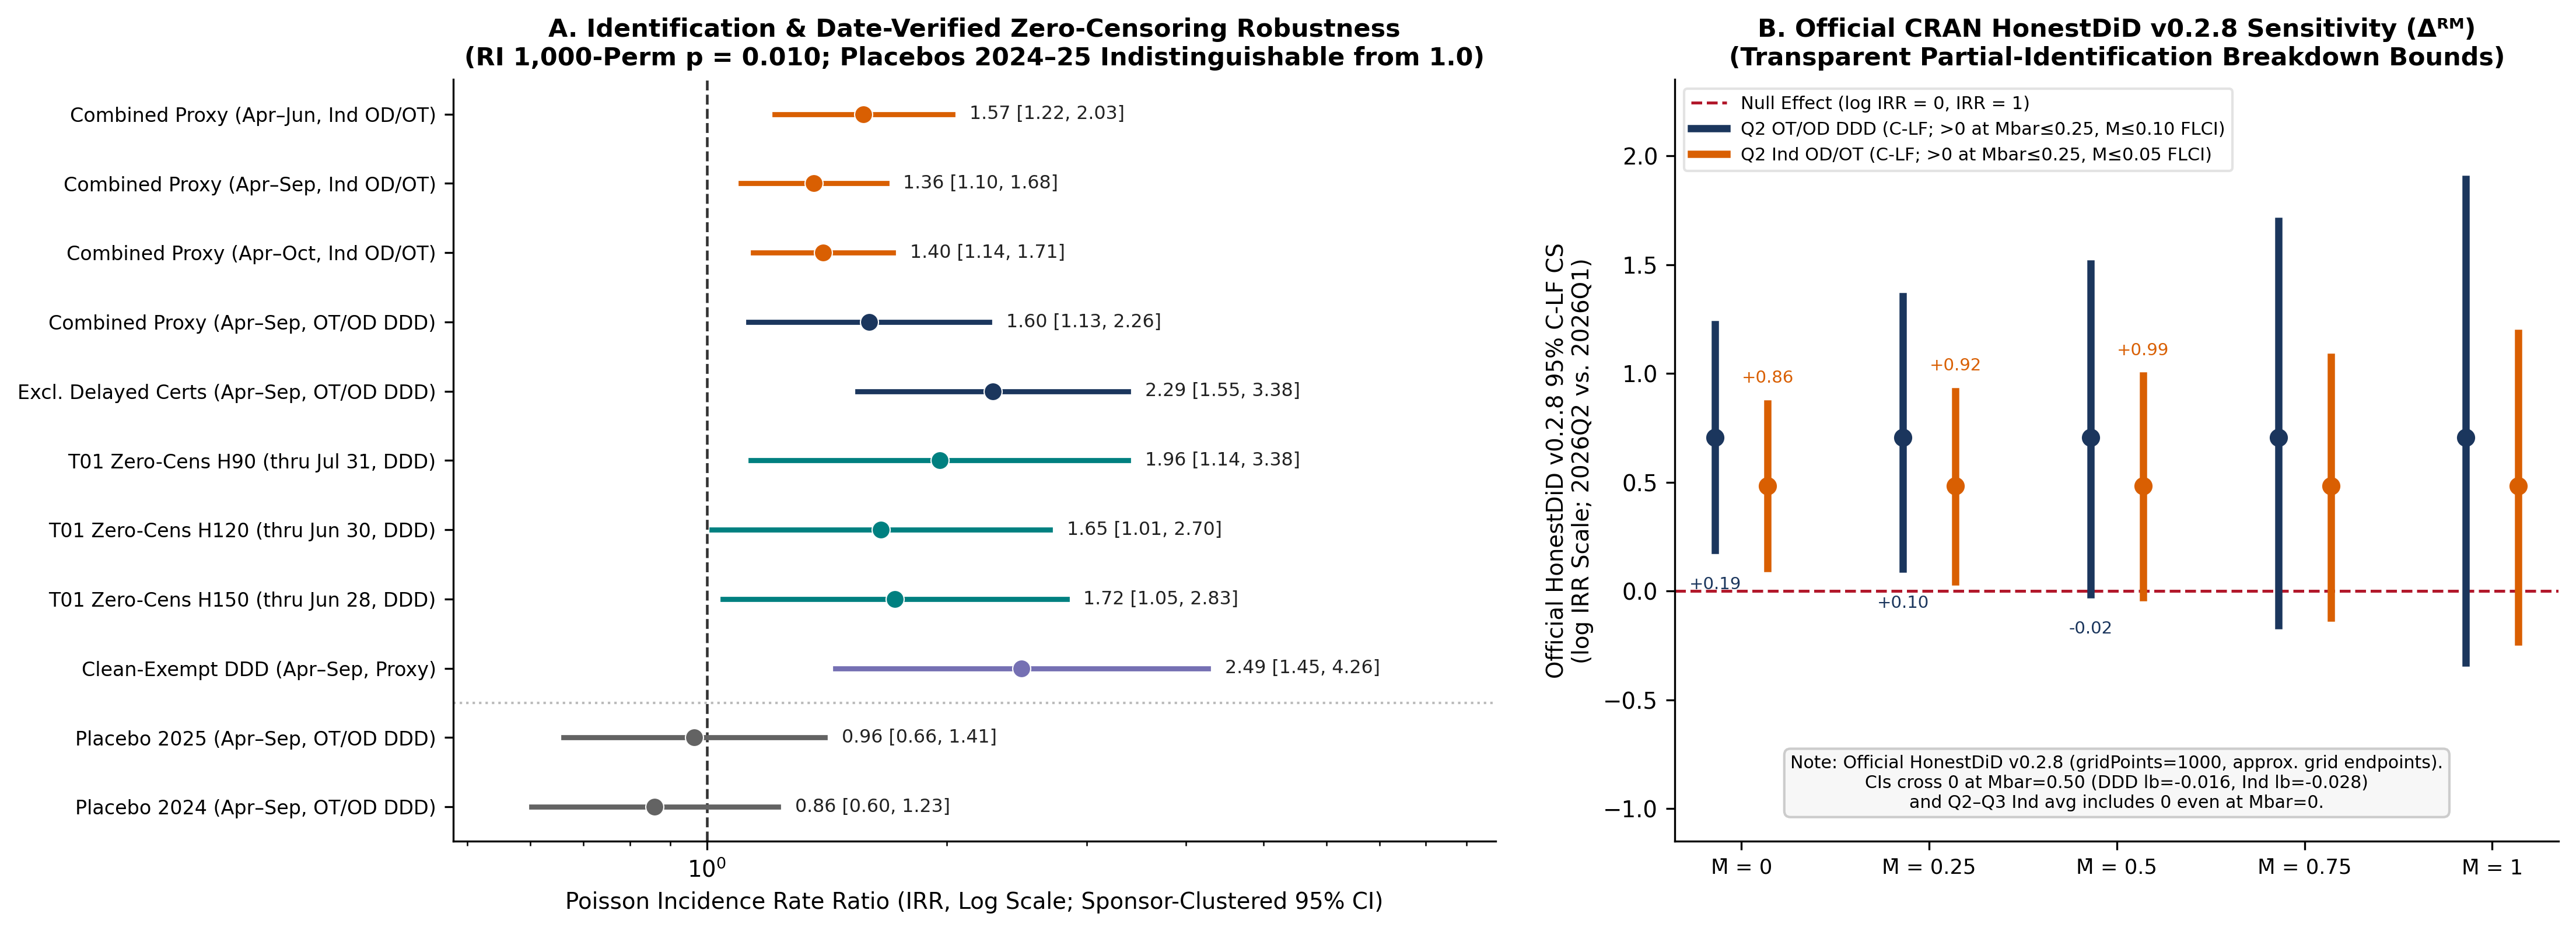
\includegraphics[width=\textwidth]{../figures/fig2_b2_identification_and_placebos.png}
\caption{\textbf{Identification Forest Plot and Official CRAN R \texttt{HonestDiD} v0.2.8 Sensitivity Bounds.} (\textbf{A}) Primary combined-proxy, certification-excluded, date-verified zero-censoring (T01), Clean-Exempt DDD, and historical placebo estimates. (\textbf{B}) Official \texttt{HonestDiD} v0.2.8 $\Delta^{RM}(\bar{M})$ C-LF 95\% confidence sets (\texttt{gridPoints=1000}, grid-resolution approximations) for 2026Q2 impact: both OT/OD DDD and Industry OD/OT exclude zero through $\bar{M}=0.25$ but cross zero at $\bar{M}=0.50$.}
\label{fig:b2_fig2}
\end{figure}

\begin{table}[H]
\centering
\caption{Official CRAN R \texttt{HonestDiD} v0.2.8 Partial-Identification Bounds (Log-IRR 95\% CS; Grid-Resolution Approximations; All 15 Specs \& T10 Expanded-Grid Audit in Supplementary Table S3).}
\label{tab:b2_honestdid}
\footnotesize
\setlength{\tabcolsep}{3.5pt}
\begin{tabularx}{\textwidth}{@{} >{\raggedright\arraybackslash}X c c c c c @{}}
\toprule
\textbf{Specification (Ref; Pre/Post)} & \textbf{$\hat{\theta}$ (IRR)} & \textbf{Original CS} & \textbf{$\Delta^{SD}$ FLCI $>0$ Thru} & \textbf{$\Delta^{RM}$ ($\bar{M}=0.25$)} & \textbf{$\Delta^{RM}$ ($\bar{M}=0.50$)} \\
\midrule
Qtrly OT/OD DDD (\texttt{26Q1}; 3/2): Q2 & $+0.705$ (2.02) & $[+0.18, +1.23]$ & $M=0.10$ ($0.15$ crosses) & $[+0.10, +1.35]^\dagger$ & $[-0.02, +1.50]$ \\
Qtrly OT/OD DDD (\texttt{26Q1}; 3/2): Q2--Q3 & $+0.758$ (2.13) & $[+0.29, +1.23]$ & $M=0.05$ ($0.10$ crosses) & $[+0.15, +1.42]^\dagger$ & $[-0.06, +1.70]$ \\
Qtrly Ind OD/OT (\texttt{26Q1}; 3/2): Q2 & $+0.482$ (1.62) & $[+0.10, +0.87]$ & $M=0.05$ ($0.10$ crosses) & $[+0.04, +0.92]^\dagger$ & $[-0.03, +0.99]$ \\
Qtrly Ind OD/OT (\texttt{26Q1}; 3/2): Q2--Q3 & $+0.326$ (1.38) & $[-0.01, +0.67]$ & $M=0.02$ ($0.05$ crosses) & $[-0.11, +0.75]^\ddagger$ & $[-0.25, +0.89]$ \\
Qtrly Within-ACT (\texttt{26Q1}; 3/2): Q2 & $+0.744$ (2.10) & $[+0.35, +1.14]$ & $M=0.30$ (Pre-trend rej.) & $[+0.23, +1.33]^\dagger$ & $[+0.06, +1.58]^\dagger$ \\
\midrule
Mthly Ind OD/OT (\texttt{26-02}; 10/8): Apr & $+0.985$ (2.68) & $[+0.36, +1.61]$ & $M=0.02$ ($0.05$ crosses) & $[+0.19, +1.86]^\dagger$ & $[-0.19, +2.24]$ \\
Mthly Ind OD/OT (\texttt{26-02}; 10/8): 6m & $+0.619$ (1.86) & $[+0.05, +1.19]$ & $M=0.00$ ($0.02$ crosses) & $[-0.65, +1.94]$ & $[-1.82, +3.00]$ \\
Mthly OT/OD DDD (\texttt{26-02}; 10/8): Apr & $+1.030$ (2.80) & $[+0.20, +1.86]$ & Crosses at $M=0$ & $[-0.09, +2.30]$ & $[-0.94, +2.98]$ \\
Mthly Ind OD/OT (\texttt{26-03}; 11/7): 6m & $+0.072$ (1.07) & $[-0.40, +0.55]$ & $M=0.00$ ($0.02$ crosses) & $[-1.13, +1.03]^\ddagger$ & $[-2.11, +1.91]$ \\
Mthly OT/OD DDD (\texttt{26-03}; 11/7): 6m & $+0.538$ (1.71) & $[-0.12, +1.19]$ & $M=0.00$ ($0.02$ crosses) & $[-1.15, +2.09]^\ddagger$ & $[-2.63, +3.58]$ \\
\bottomrule
\end{tabularx}
\par\smallskip\raggedright\footnotesize
$^\dagger$Excludes 0 at 95\% confidence. $^\ddagger$Already includes 0 at $\bar{M}=0$. Computed with official CRAN R \texttt{HonestDiD} v0.2.8 (R 4.5.3; \texttt{BCdata} vignette verified). Monthly \texttt{ref=2026-02} specs retain \texttt{2026-03} at $t=+1$ ($l_1=0$). \textbf{T10 Grid Audit:} All 5 outer-$\bar{M}$ entries hitting the default $\pm 20\,\mathrm{SE}$ bound (Qtrly Within-ACT Q2--Q3 $\bar{M}=2$ and 4 monthly 6m averages at $\bar{M}=1$; all already containing 0) were recomputed on $\pm 40\,\mathrm{SE}$ (1,001 pts, both boundaries rejected; 0/15 remaining hits in Table S3). C-LF bounds are discrete-grid approximations (monthly default step $0.11$--$0.15$; expanded step $0.015$--$0.029$).
\end{table}

Table~\ref{tab:b2_honestdid} establishes a sharp partial-identification boundary: \textbf{our quasi-experimental estimates survive modest parallel-trends violations ($\bar{M}\le 0.25$ on quarterly Q2 impact and April on-impact Industry OD/OT), but are NOT robust to larger post-treatment trend breaks.} At $\bar{M}=0.50$, both quarterly 2026Q2 DDD ($[-0.016, +1.505]$) and Industry OD/OT ($[-0.028, +0.988]$) cross zero; quarterly Q2--Q3 Industry OD/OT average includes zero even at $\bar{M}=0$ ($[-0.010, +0.663]$); and March-referenced monthly averages include zero because March 2026 had already bounced upward from the January--February trough.

\subsection{Organizational Mechanisms, Stale-Data Decay, and Phase-1 Spillover}
Figure~\ref{fig:b2_fig3} decomposes post-sweep Industry and Academic responses (combined tracking proxy, Apr--Sep 2026 vs.\ Clean Exempt controls) across portfolio size, delinquency cohort age, backlog size, and exempt Phase 1 spillovers:
\begin{itemize}
    \item \textbf{Small-Sponsor Catch-Up vs.\ Large-Pharma Baseline (Panel A):} Once unposted tracking is recovered, the post-sweep corporate lift is concentrated in \textbf{small commercial sponsors (1--2 FDA trials)} ($\mathrm{IRR}=1.841$ $[1.327, 2.554]$, $p=0.00026$; hazard $1.80\%\to 2.99\%$), whereas mid-size ($3$--$19$: $1.297$ $[0.925, 1.819]$, $p=0.132$) and large firms ($20+$: $1.090$ $[0.745, 1.595]$, $p=0.657$) show no statistically detectable incremental lift (large pharma already maintained an $8.22\%/\text{mo}$ pre-sweep rate). Academic sponsors show no statistically detectable lift across any portfolio tier (Small $1.439$, $p=0.092$; Mid $0.939$, $p=0.782$; Large $0.985$, $p=0.929$).
    \item \textbf{Stale-Data Decay Cliff (Panel B):} Significant corporate compliance gains appear in \textbf{recently overdue 2023--2025 cohorts} ($\mathrm{IRR}=1.500$ $[1.185, 1.898]$, $p=0.00074$; $3.89\%\to 5.65\%$), with no statistically detectable lift in 2021--2022 ($1.253$ $[0.694, 2.261]$, $p=0.455$) or legacy 2017--2020 cohorts ($0.913$ $[0.362, 2.301]$, $p=0.847$).
    \item \textbf{Backlog Gradient \& No Detectable Phase-1 Spillover (Panel C):} Corporate sponsors responded across all delinquent backlog tiers ($1$ trial: $\mathrm{IRR}=2.961$, $p=2.6\times 10^{-7}$; $2$--$4$ trials: $2.826$, $p=7.6\times 10^{-6}$; $5+$ trials: $2.029$, $p=0.0094$), whereas multi-trial academic sponsors showed no detectable lift ($2$--$4$: $1.197$, $p=0.397$; $5+$: $0.866$, $p=0.683$; single-trial academic $2.072$, $p=0.00035$). Testing within-firm spillover to \textbf{statutorily exempt U.S.\ Phase 1 trials} ($n=3,910$ trials, 125 events) yields \textbf{no statistically detectable spillover} ($\mathrm{IRR}=0.893$, 95\% CI $[0.407, 1.957]$, $p=0.777$), though the wide confidence interval cannot exclude modest spillovers. We explicitly retract our pre-audit raw-April Phase-1 spillover claim.
\end{itemize}

\begin{figure}[H]
\centering
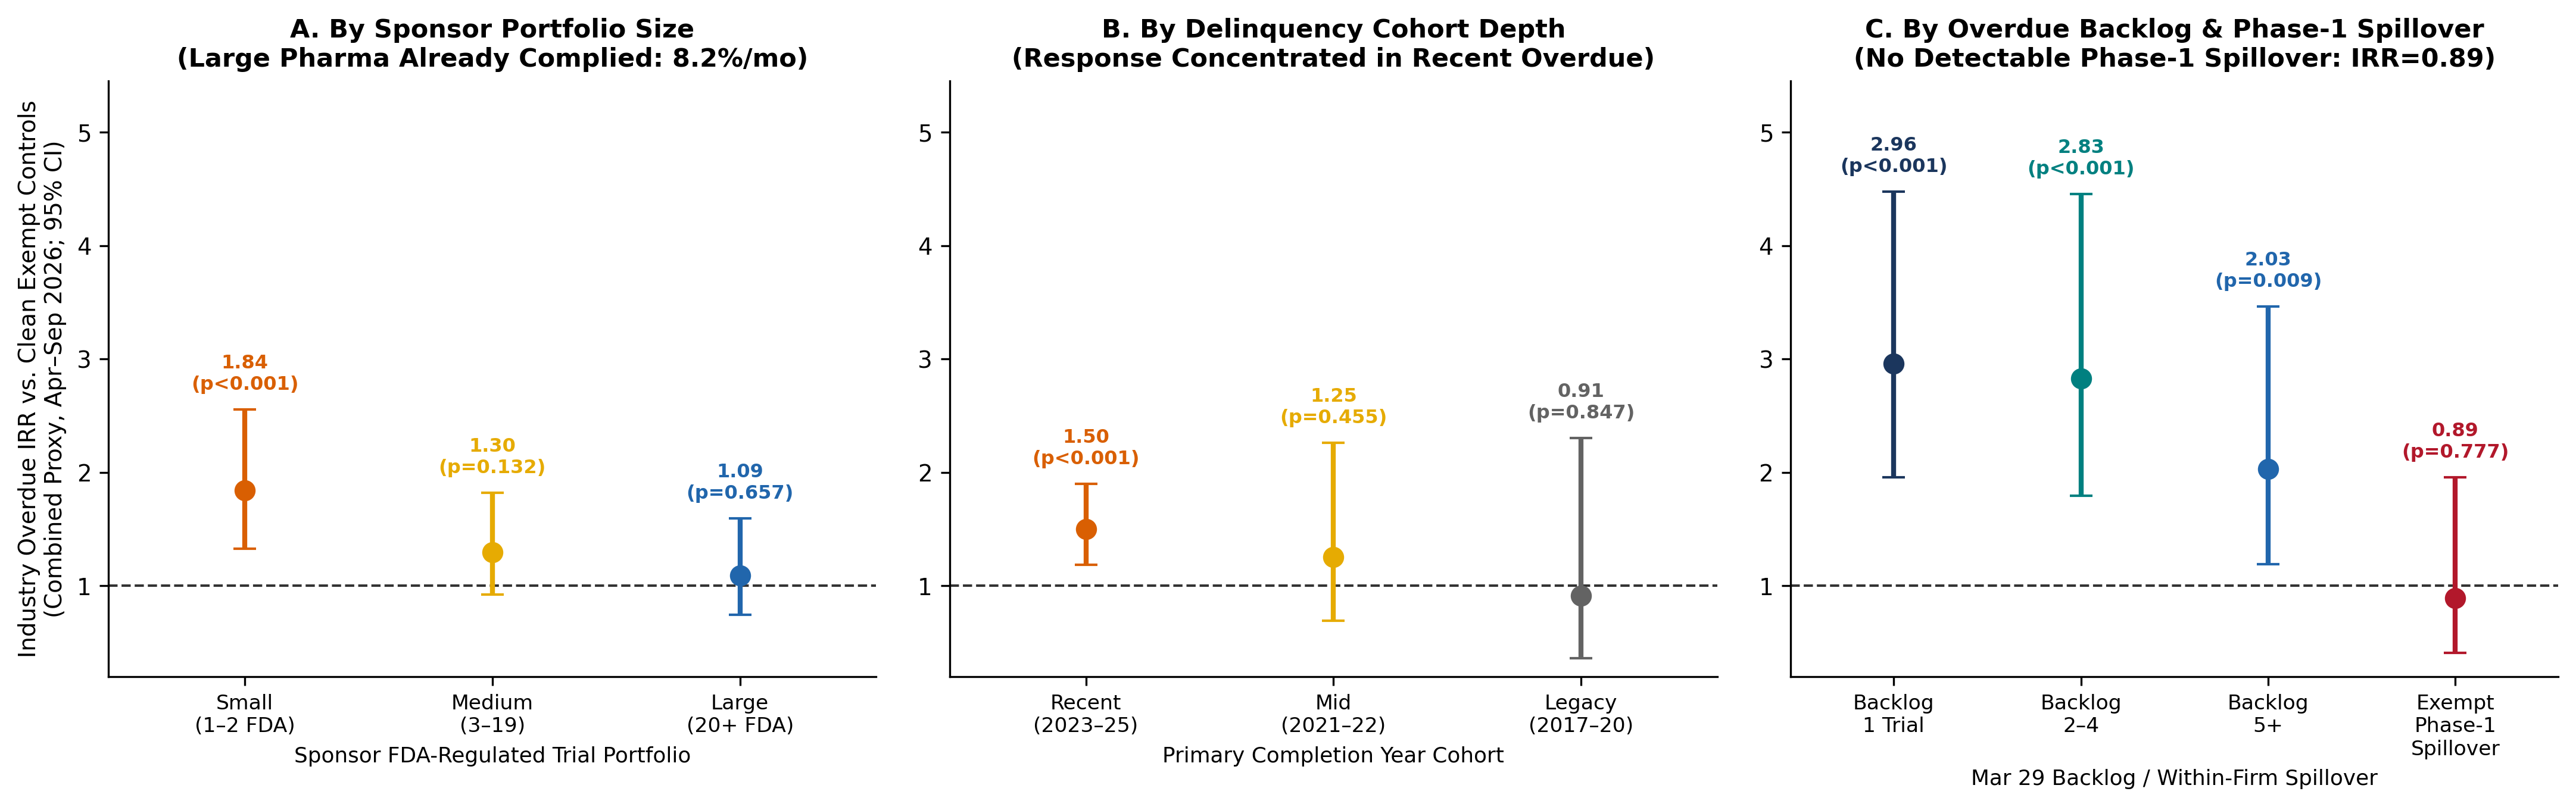
\includegraphics[width=\textwidth]{../figures/fig3_b2_governance_mechanisms.png}
\caption{\textbf{Governance Mechanisms and Exempt Phase-1 Spillover Audit (Combined Tracking Proxy, Apr--Sep 2026).} (\textbf{A}) Lift concentrates in small commercial sponsors while large pharma already operates near an 8.2\%/mo baseline. (\textbf{B}) Significant lift appears in 2023--2025 cohorts, with no detectable lift in 2017--2020 legacy trials ($0.91$ $[0.36, 2.30]$). (\textbf{C}) Multi-trial industry backlogs respond across all tiers, while within-firm spillover to exempt Phase 1 trials is not statistically detectable ($\mathrm{IRR}=0.89$ $[0.41, 1.96]$, $p=0.777$).}
\label{fig:b2_fig3}
\end{figure}

\subsection{H4 Clinical Outcome Audit \& Exploratory Power Boundaries (T03/T04)}
Table~\ref{tab:b2_h4} and Figure~\ref{fig:b2_fig4} audit full clinical outcomes across all 5,064 U.S.\ FDA-regulated results disclosures (2024--2026: 2,822 on-time, 1,930 pre-sweep overdue, 312 post-sweep overdue), reporting within-sponsor fixed-effects estimates alongside 80\%-power MDEs, \textbf{post-hoc exploratory} $\pm 5$ pp / $\pm 10$ pp TOST margin sensitivities, and QC-backlog selection checks.

\begin{table}[H]
\centering
\caption{Within-Sponsor Fixed-Effects H4 Clinical Outcome Audit with 80\%-Power MDEs and Post-Hoc Exploratory TOST Margin Sensitivities ($n=4,224$ Trials Across 555 Sponsors; Efficacy Subsample $n=1,035$ Across 184 Sponsors).}
\label{tab:b2_h4}
\footnotesize
\setlength{\tabcolsep}{3.5pt}
\begin{tabularx}{\textwidth}{@{} >{\raggedright\arraybackslash}X c c c c >{\raggedright\arraybackslash}p{1.25in} @{}}
\toprule
\textbf{Clinical Outcome} & \textbf{$n$ (Spon.)} & \textbf{FE Diff (pp) [95\% CI]} & \textbf{$\mathrm{MDE}_{80}$} & \textbf{Post-Hoc TOST $\pm 5/\pm 10$} & \textbf{Inferential Boundary} \\
\midrule
All-Cause Mortality & 4,180 (553) & $+0.71$ $[-2.11, +3.53]$ & 4.03 & 0.0014 / $<0.0001$ & Within post-hoc $\pm 5$ pp margin \\
Serious Adverse Events & 4,179 (554) & $+0.39$ $[-2.68, +3.45]$ & 4.38 & 0.0016 / $<0.0001$ & Within post-hoc $\pm 5$ pp margin \\
Early Termination & 4,224 (555) & $-1.89$ $[-8.92, +5.14]$ & 10.05 & 0.193 / 0.0119 & Inside $\pm 10$ pp only \\
Omitted Primary $p$-Val & 4,224 (555) & $-4.79$ $[-11.78, +2.21]$ & 10.00 & 0.476 / 0.072 & Moderate uncertainty \\
Primary $p\ge 0.05$ (Null) & 1,035 (184) & $-0.14$ $[-16.13, +15.85]$ & \textbf{22.86} & 0.276 / 0.113 & \textbf{Severely underpowered} \\
\bottomrule
\end{tabularx}
\par\smallskip\raggedright\footnotesize
Note: $\pm 5$ pp and $\pm 10$ pp TOST margins are \textbf{post-hoc exploratory sensitivity margins} chosen after observing initial CIs, not pre-specified clinical equivalence thresholds. Analysis covers disclosed trials only and does not exclude strategic concealment among still-unposted or never-submitted trials.
\end{table}

\begin{figure}[H]
\centering
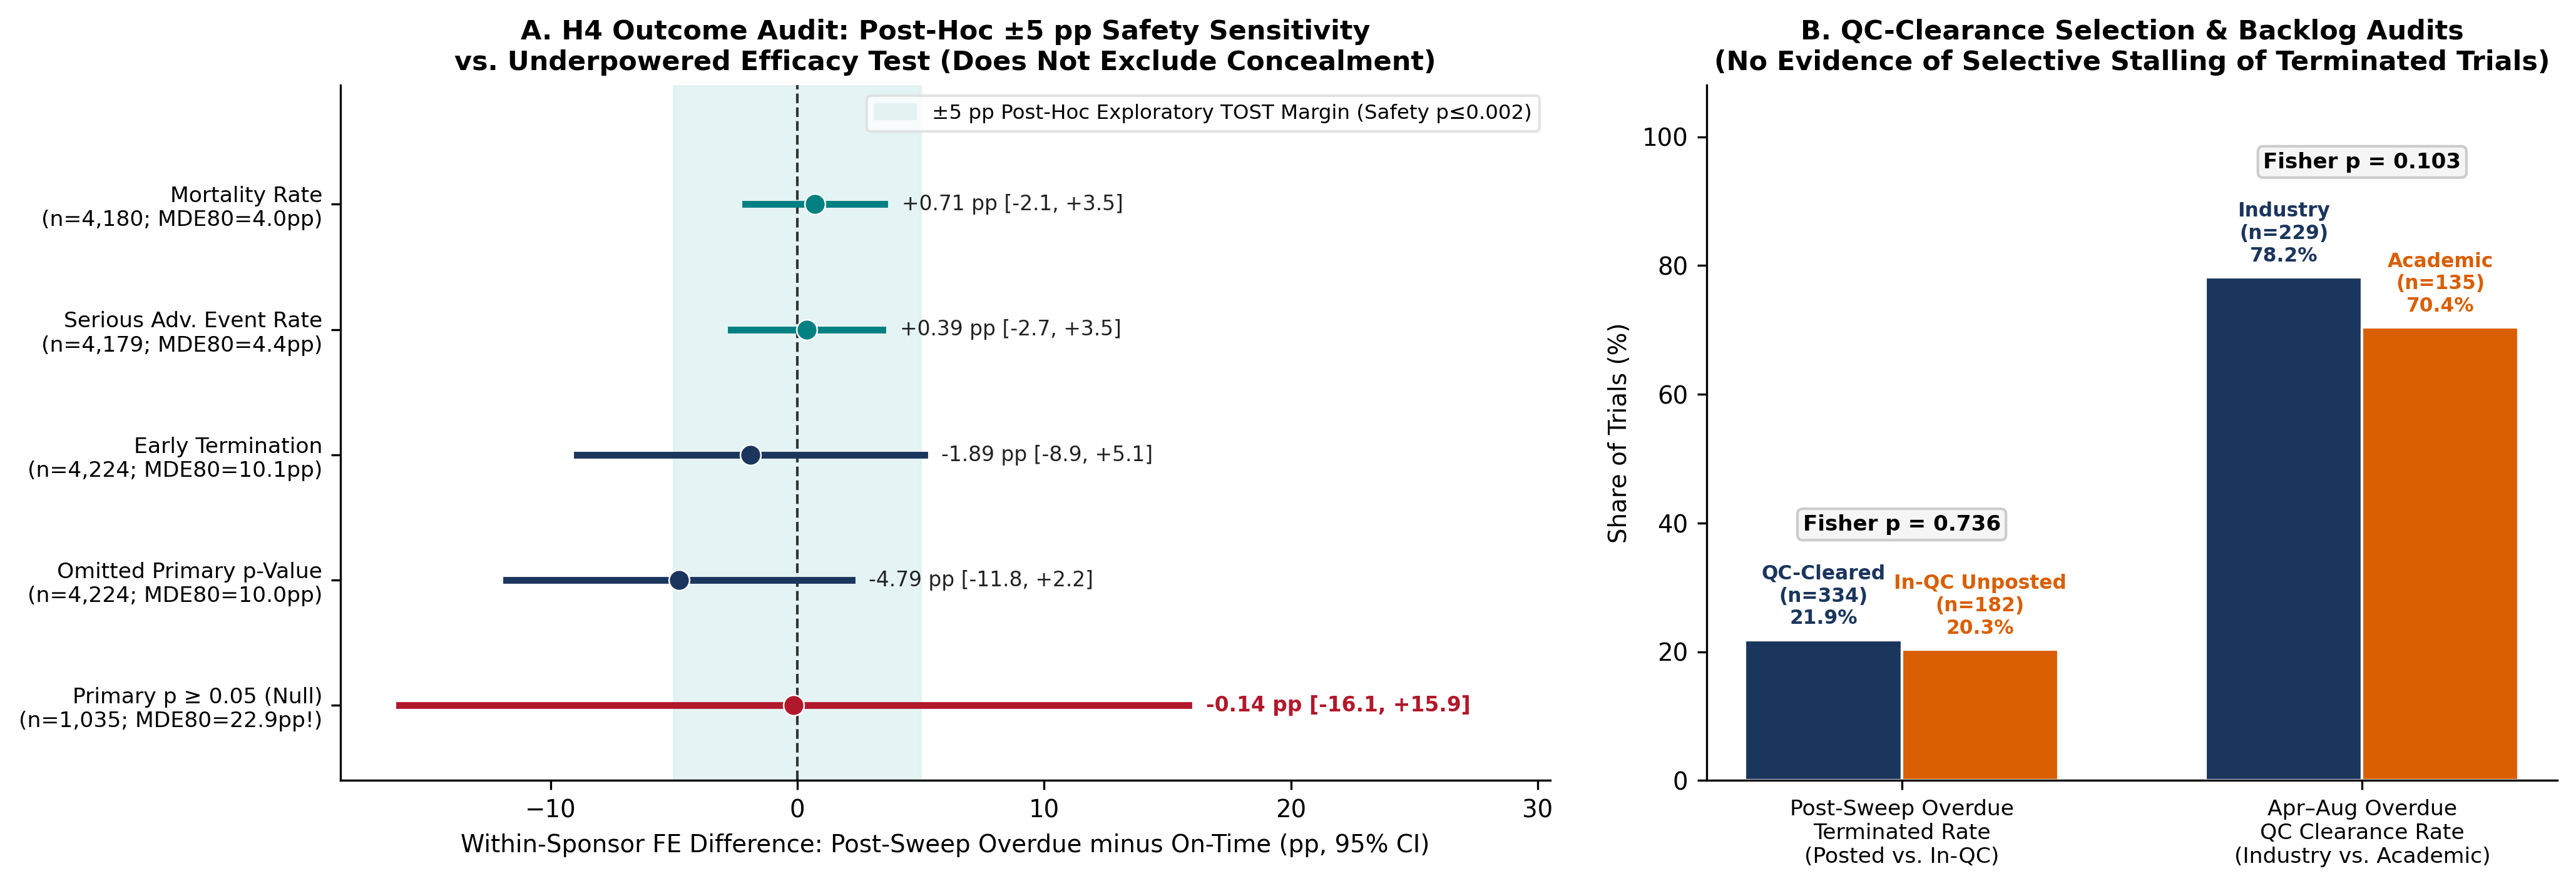
\includegraphics[width=\textwidth]{../figures/fig4_b2_lemons_vs_inattention.png}
\caption{\textbf{H4 Clinical Outcome Audit (Post-Hoc Exploratory TOST Margins) and QC-Clearance Selection Checks.} (\textbf{A}) Within-sponsor FE differences lie inside post-hoc exploratory $\pm 5$ pp margins for mortality and SAE rates, while primary efficacy non-significance has a wide, underpowered 95\% CI ($[-16.1, +15.9]$ pp, $\mathrm{MDE}_{80}=22.9$ pp); neither rules out strategic hiding in undisclosed trials. (\textbf{B}) Unposted in-QC trials show no statistically detectable excess early termination ($p=0.736$) and post-sweep QC clearance does not differ significantly across sectors ($p=0.103$).}
\label{fig:b2_fig4}
\end{figure}

Within sponsors, observed post-sweep overdue disclosures lie inside post-hoc exploratory $\pm 5$ pp sensitivity margins for mortality ($+0.71$ pp $[-2.11, +3.53]$, exploratory TOST $p=0.0014$) and SAE rates ($+0.39$ pp $[-2.68, +3.45]$, $p=0.0016$), and show no excess early termination beyond $\pm 10$ pp ($-1.89$ pp, exploratory TOST $p=0.0119$). Unposted in-QC post-sweep overdue trials ($n=182$, 20.33\% terminated) show no statistically detectable excess termination relative to QC-cleared post-sweep overdue trials ($n=334$, 21.86\% terminated, Fisher $p=0.736$), and April--August overdue QC clearance rates do not differ significantly between Industry (78.17\%, $n=229$) and Academic (70.37\%, $n=135$, Fisher $p=0.103$). However, because 69.9\%--74.2\% of results omit formal primary p-values, the within-sponsor efficacy subsample shrinks to $n=1,035$ trials (only 94 post-sweep overdue), yielding a 95\% CI of $[-16.13, +15.85]$ pp ($\mathrm{MDE}_{80}=22.86$ pp). We therefore \textbf{explicitly retract} any broad claim of ``falsifying the strategic lemons hypothesis'': the observed safety CIs are narrow on posted disclosures, but the efficacy test is uninformative regarding moderate ($\pm 10$--$15$ pp) hiding and observed outcomes cannot exclude strategic concealment among trials that remained unsubmitted after the sweep.

\section{Discussion, Policy Implications, and Scientific Boundaries}
The March 30, 2026 FDA outreach illustrates both the scope and limits of low-cost administrative reminders. Relative to contemporaneous on-time ACTs and academic sponsors, commercial sponsors increased overdue submission hazards by 36\%--60\%, concentrated among small commercial firms (1--2 trials) and recently overdue 2023--2025 studies where trial teams and analytical datasets remain intact. Conversely, we detect no statistically significant response among multi-trial academic medical centers, legacy 2017--2020 commercial records, or statutorily exempt Phase 1 trials.

\textbf{Explicit Scientific Boundaries and Limitations:}
\begin{enumerate}
    \item \textbf{Partial-Identification \& Grid-Resolution Limits (T06/T10):} Under official CRAN R \texttt{HonestDiD} v0.2.8, quarterly 2026Q2 effects survive $\Delta^{RM}(\bar{M}\le 0.25)$ and $\Delta^{SD}(M\le 0.05$--$0.10)$, but cross zero at $\bar{M}=0.50$, and quarterly Q2--Q3 Industry OD/OT average plus March-referenced monthly averages include zero even at $\bar{M}=0$. All C-LF intervals are discrete-grid approximations (monthly default step $0.11$--$0.15$; 5 outer-$\bar{M}$ boundary-hitting entries recomputed on $\pm 40\,\mathrm{SE}$ with 1,001 points, step $0.015$--$0.029$, both boundaries rejected).
    \item \textbf{Within-ACT Pre-Trend Failure:} Raw Within-ACT Industry-vs.-Academic overdue DiD violates monthly pre-trends ($p=0.00037$) and is imprecise in short 3--4m windows once unposted April academic records are recovered; primary identification relies on Overdue-vs.-On-Time designs.
    \item \textbf{Proxy-Date \& Non-Observation Boundaries:} Although \path{estimatedResultsFirstSubmitDate} matched \path{earliest_subinfo_release_date} on 100.0\% of 2,026 records with zero certification mixing, very recent November submissions not yet entered into tracking cannot be observed; similarly, zero observed post-sweep delayed certifications does not prove the absence of other administrative deferral practices, and wide CIs on Phase 1 ($[0.41, 1.96]$) and legacy cohorts ($[0.36, 2.30]$) mean ``not statistically detectable'' rather than exact zero.
    \item \textbf{Unobserved Recipient Roster:} FDA did not publish recipient identities \citep{fda2026bulletin}; estimates represent intent-to-treat (ITT) effects across statutorily overdue ACTs.
    \item \textbf{Post-Hoc TOST \& Undisclosed-Trial Selection (T03/T04):} The $\pm 5$ pp / $\pm 10$ pp TOST margins are post-hoc exploratory sensitivities rather than pre-specified clinical equivalence tests; primary efficacy non-significance ($\mathrm{MDE}_{80}=22.86$ pp) is severely underpowered; and observed disclosures cannot rule out strategic concealment among trials that remained undisclosed.
\end{enumerate}

\section*{Data and Code Availability}
{\sloppy
All raw ClinicalTrials.gov REST API v2 snapshots, forensic T00--T10 audit JSONs, official CRAN R \texttt{HonestDiD} v0.2.8 output (\path{audit/b2_t06_official_r_honestdid_results.json}), T10 expanded-grid audit (\path{audit/b2_t10_grid_boundary_and_convergence_audit.json}), Supplementary CSV tables (\path{audit/b2_supp_monthly_combined_proxy_hazards.csv}, \path{audit/b2_supp_t00_t07_master_estimates.csv}, \path{audit/b2_supp_t06_official_r_honestdid_all15.csv}), post-pilot analysis plan (\path{PREREG_B2.md}), and runnable Python and R replication scripts are archived in \path{studies/study_b2_fda_2026_sweep/}.\par}

\bibliographystyle{unsrtnat}
\bibliography{references_b2}
\end{document}
